\documentclass[tikz,border=5mm]{standalone}
\usepackage{tikz}
\usetikzlibrary{shapes.geometric, shapes.multipart, arrows.meta, positioning, calc, fit, backgrounds, shadows, decorations.pathreplacing, matrix, patterns}

% Color Definitions
\definecolor{host_bg}{RGB}{255,250,230}
\definecolor{host_border}{RGB}{200,150,50}
\definecolor{l1_bg}{RGB}{230,240,255}
\definecolor{l1_border}{RGB}{50,100,200}
\definecolor{l1_inner_bg}{RGB}{245,250,255}
\definecolor{l2_bg}{RGB}{230,255,230}
\definecolor{l2_border}{RGB}{50,150,50}
\definecolor{l2_inner_bg}{RGB}{245,255,245}
\definecolor{l3_bg}{RGB}{255,230,230}
\definecolor{l3_border}{RGB}{200,50,50}
\definecolor{l3_inner_bg}{RGB}{255,245,245}
\definecolor{bus_color}{RGB}{80,80,80}
\definecolor{warp_text}{RGB}{100,0,100}

\begin{document}
    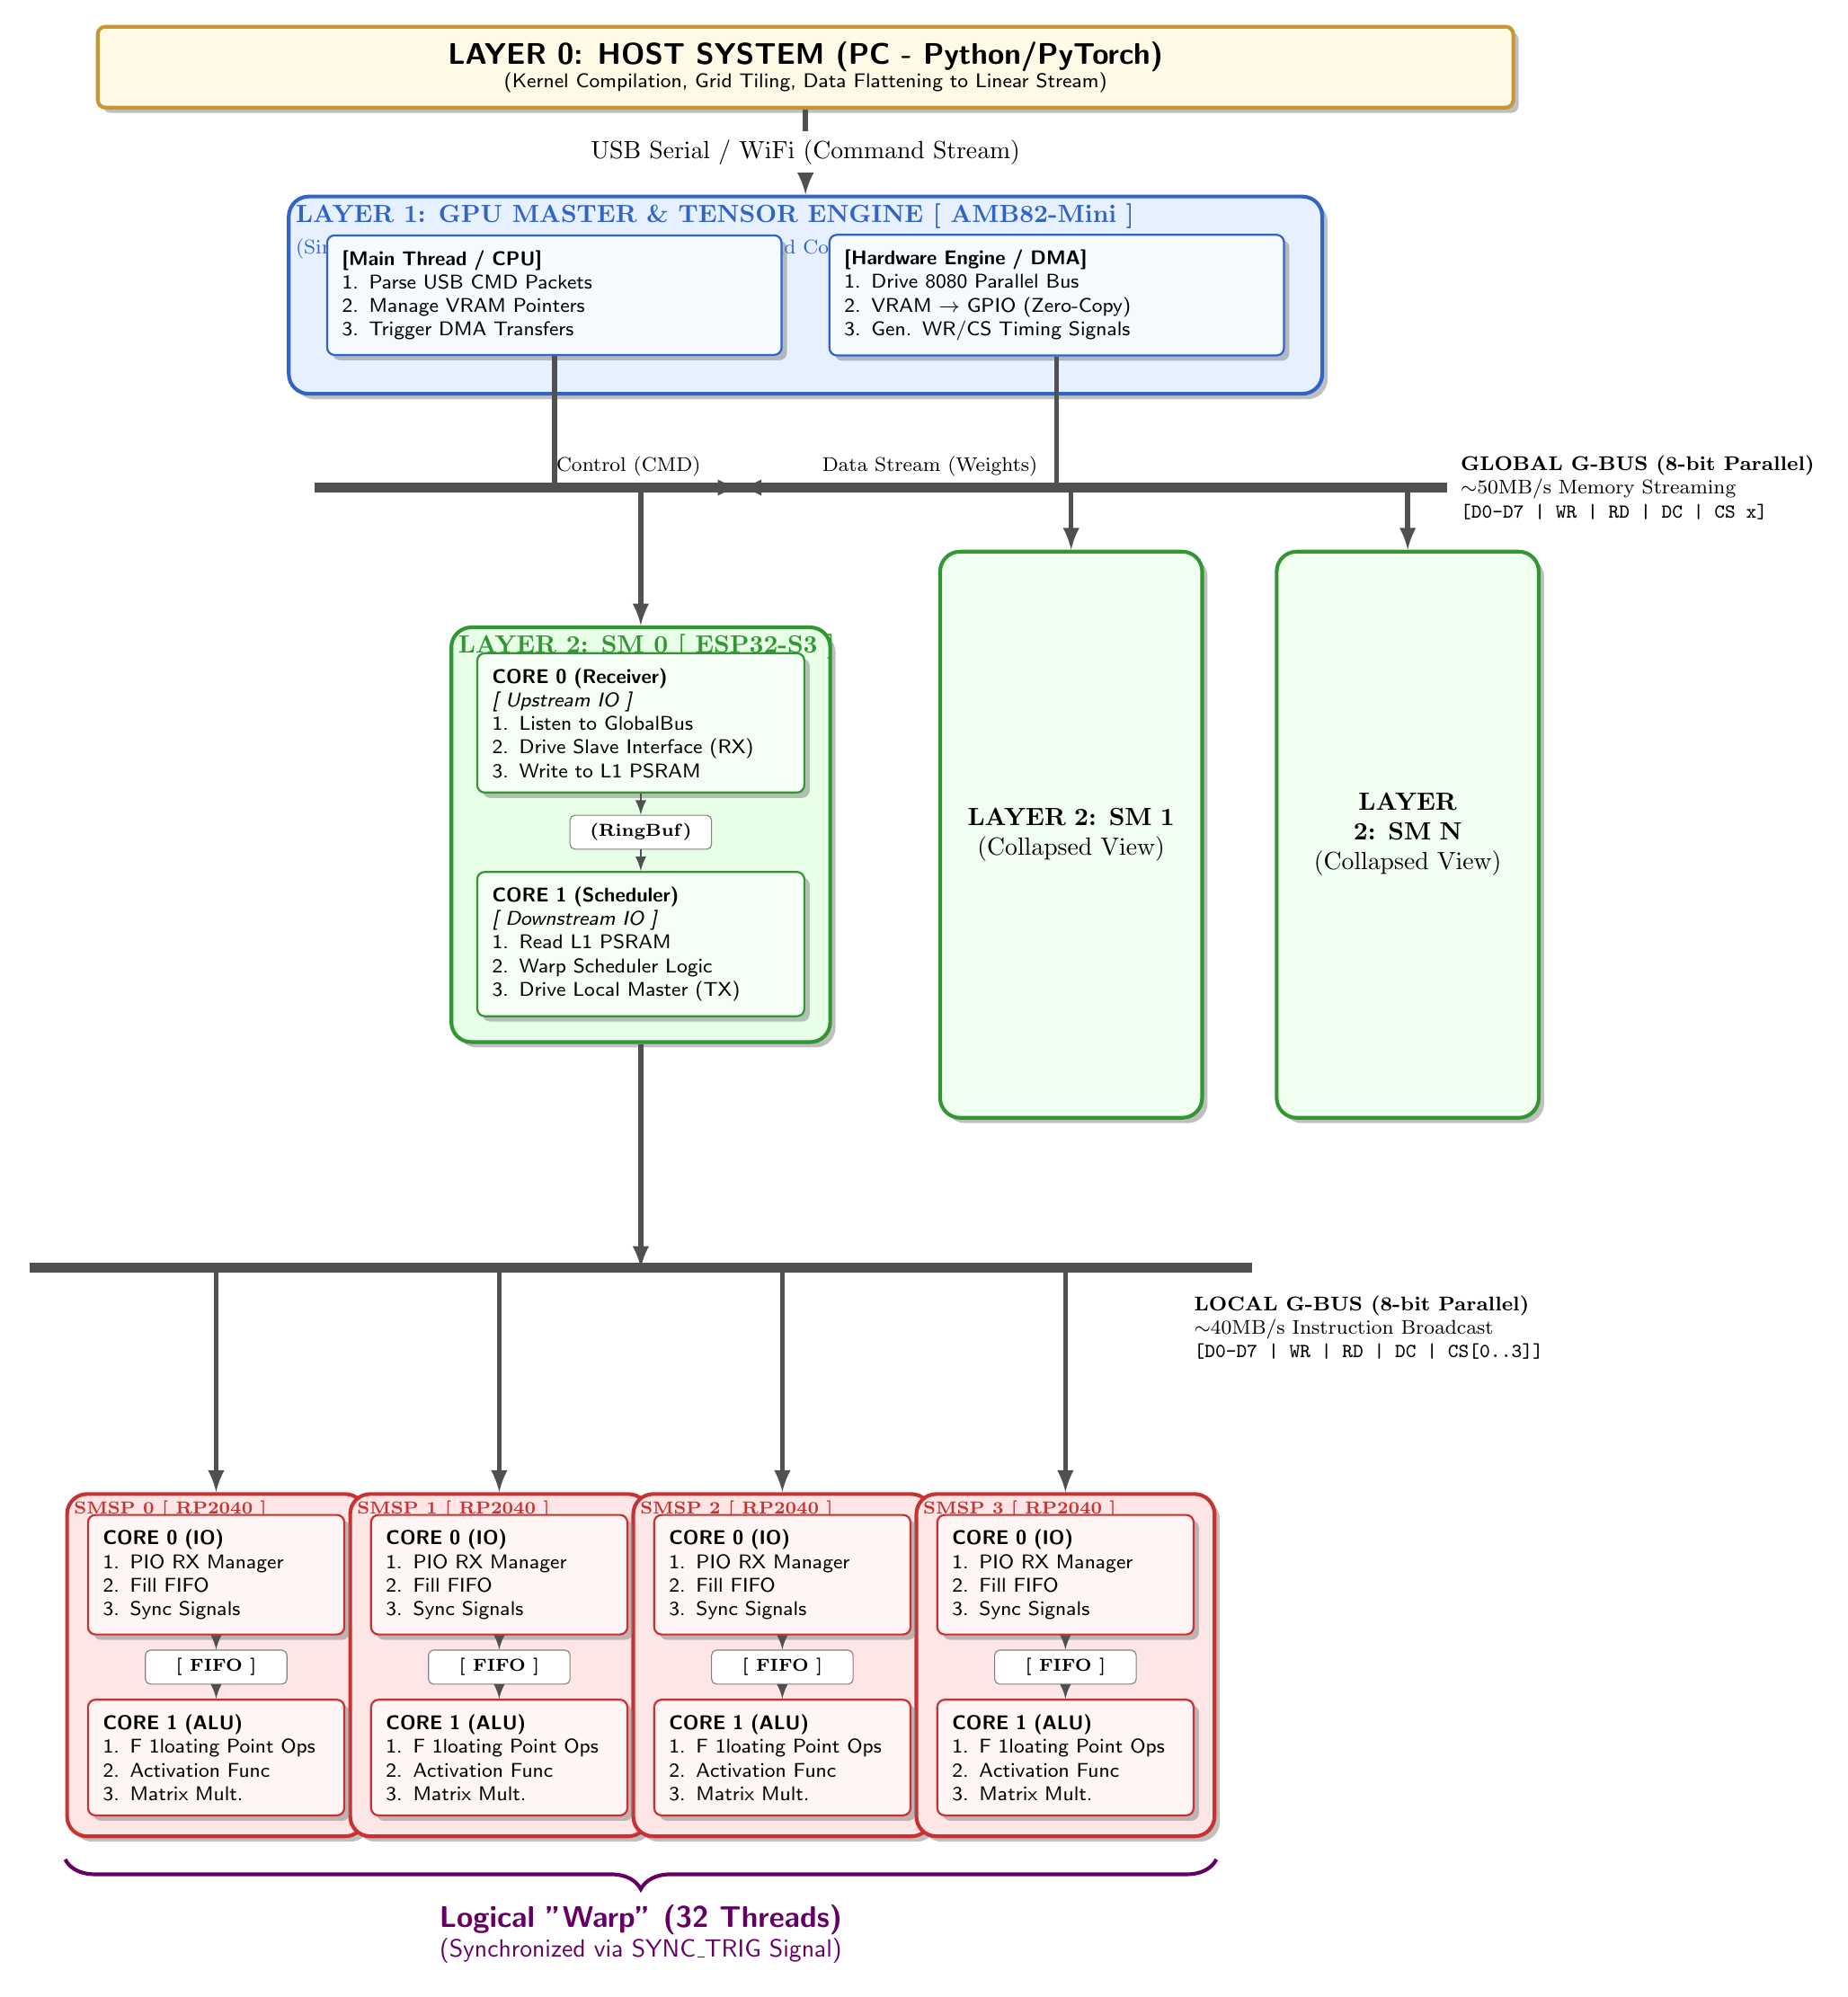
\begin{tikzpicture}[
        node distance=1.5cm, 
        % --- Styles ---
        base_box/.style={
            rectangle, draw, rounded corners=3pt, align=left, drop shadow,
            font=\sffamily\footnotesize, inner sep=6pt
        },
        % Layer Containers
        host_box/.style={base_box, draw=host_border, fill=host_bg, line width=1.5pt, align=center},
        l1_cont/.style={draw=l1_border, fill=l1_bg, rounded corners=8pt, line width=1.5pt, inner sep=15pt, drop shadow},
        l2_cont/.style={draw=l2_border, fill=l2_bg, rounded corners=8pt, line width=1.5pt, inner sep=10pt, drop shadow},
        l3_cont/.style={draw=l3_border, fill=l3_bg, rounded corners=8pt, line width=1.5pt, inner sep=8pt, drop shadow},
        % Internal Modules (White/Light boxes)
        l1_node/.style={base_box, draw=l1_border, fill=l1_inner_bg, text width=6.0cm, line width=0.8pt},
        l2_node/.style={base_box, draw=l2_border, fill=l2_inner_bg, text width=4.2cm, line width=0.8pt},
        l3_node/.style={base_box, draw=l3_border, fill=l3_inner_bg, text width=3.2cm, line width=0.8pt},
        fifo_node/.style={rectangle, draw=gray, fill=white, rounded corners=2pt, font=\scriptsize\bfseries, align=center, minimum width=2cm},
        % Lines
        bus_line/.style={draw=bus_color, line width=2pt, -latex},
        thin_line/.style={draw=bus_color, line width=1pt, -latex},
        % Style for the underbrace
        warp_brace/.style={decorate, decoration={brace, amplitude=12pt, mirror}, line width=1.5pt, draw=warp_text}
    ]

    % =========================================================================
    % LAYER 0: HOST SYSTEM
    % =========================================================================
    \node[host_box, minimum width=20cm] (host) {
        \textbf{\large LAYER 0: HOST SYSTEM (PC - Python/PyTorch)}\\
        (Kernel Compilation, Grid Tiling, Data Flattening to Linear Stream)
    };

    % =========================================================================
    % LAYER 1: AMB82-Mini (Dual Logic)
    % =========================================================================
    \node[below=2.5cm of host] (l1_center_helper) {};

    \node[l1_node, left=0.2cm of l1_center_helper] (l1_cpu) {
        \textbf{[Main Thread / CPU]}\\
        1. Parse USB CMD Packets\\
        2. Manage VRAM Pointers\\
        3. Trigger DMA Transfers
    };
    
    \node[l1_node, right=0.2cm of l1_center_helper] (l1_dma) {
        \textbf{[Hardware Engine / DMA]}\\
        1. Drive 8080 Parallel Bus\\
        2. VRAM $\to$ GPIO (Zero-Copy)\\
        3. Gen. WR/CS Timing Signals
    };

    \begin{scope}[on background layer]
        \node[l1_cont, fit=(l1_cpu)(l1_dma)] (l1_container) {};
        \node[anchor=north west, text=l1_border, font=\bfseries] at (l1_container.north west) {LAYER 1: GPU MASTER \& TENSOR ENGINE [ AMB82-Mini ]};
        \node[anchor=north west, text=l1_border, font=\footnotesize] at ($(l1_container.north west)+(0,-0.5)$) {(Single-core M33, utilizing DMA HW as a virtual 2nd Core)};
    \end{scope}

    \draw[bus_line] (host.south) -- node[midway, fill=white] {USB Serial / WiFi (Command Stream)} (l1_container.north);

    % =========================================================================
    % LAYER 2: ESP32-S3 (Dual Core Vertical)
    % =========================================================================
    \node[below=4.5cm of l1_container.south west, xshift=5cm] (sm0_center) {};

    \node[l2_node] (sm0_core0) at (sm0_center) {
        \textbf{CORE 0 (Receiver)}\\
        \textit{[ Upstream IO ]}\\
        1. Listen to GlobalBus\\
        2. Drive Slave Interface (RX)\\
        3. Write to L1 PSRAM
    };
    
    \node[fifo_node, below=0.3cm of sm0_core0] (sm0_ring) {(RingBuf)};
    
    \node[l2_node, below=0.3cm of sm0_ring] (sm0_core1) {
        \textbf{CORE 1 (Scheduler)}\\
        \textit{[ Downstream IO ]}\\
        1. Read L1 PSRAM\\
        2. Warp Scheduler Logic\\
        3. Drive Local Master (TX)
    };

    \begin{scope}[on background layer]
        \node[l2_cont, fit=(sm0_core0)(sm0_ring)(sm0_core1)] (sm0_container) {};
        \node[anchor=north west, text=l2_border, font=\bfseries] at (sm0_container.north west) {LAYER 2: SM 0 [ ESP32-S3 ]};
    \end{scope}

    \draw[thin_line] (sm0_core0) -- (sm0_ring);
    \draw[thin_line] (sm0_ring) -- (sm0_core1);

    % --- SM 1 & SM N (Collapsed) ---
    \node[l2_cont, right=1.5cm of sm0_container, minimum height=8cm, text width=3cm, align=center, fill=l2_bg!60] (sm1_container) {
        \textbf{LAYER 2: SM 1}\\(Collapsed View)
    };
    \node[l2_cont, right=1.0cm of sm1_container, minimum height=8cm, text width=3cm, align=center, fill=l2_bg!60] (smn_container) {
        \textbf{LAYER 2: SM N}\\(Collapsed View)
    };

    % =========================================================================
    % GLOBAL BUS (L1 -> L2)
    % =========================================================================
    \coordinate (gbus_y) at ($(l1_container.south)!0.4!(sm0_container.north)$);
    
    \draw[bus_line] (l1_cpu.south) |- (gbus_y) node[pos=0.7, above, font=\footnotesize] {Control (CMD)};
    \draw[bus_line] (l1_dma.south) |- (gbus_y) node[pos=0.7, above, font=\footnotesize] {Data Stream (Weights)};
    
    \draw[line width=4pt, draw=bus_color] ($(gbus_y) + (-6,0)$) -- ($(gbus_y) + (10,0)$) 
        node[right, align=left, font=\footnotesize] {
            \textbf{GLOBAL G-BUS (8-bit Parallel)}\\
            $\sim$50MB/s Memory Streaming\\
            \texttt{[D0-D7 | WR | RD | DC | CS x]}
        };
    
    \draw[bus_line] (gbus_y -| sm0_container.north) -- (sm0_container.north);
    \draw[bus_line] (gbus_y -| sm1_container.north) -- (sm1_container.north);
    \draw[bus_line] (gbus_y -| smn_container.north) -- (smn_container.north);

    % =========================================================================
    % LAYER 3: RP2040 (Dual Core Vertical)
    % =========================================================================
    
    % Macro for drawing SMSP
    \newcommand{\drawSMSP}[3]{
        \node[l3_node] (#1_core0) at (#2) {
            \textbf{CORE 0 (IO)}\\
            1. PIO RX Manager\\
            2. Fill FIFO\\
            3. Sync Signals
        };
        \node[fifo_node, below=0.2cm of #1_core0] (#1_fifo) {[ FIFO ]};
        \node[l3_node, below=0.2cm of #1_fifo] (#1_core1) {
            \textbf{CORE 1 (ALU)}\\
            1. F 1loating Point Ops\\
            2. Activation Func\\
            3. Matrix Mult.
        };
        
        \begin{scope}[on background layer]
            \node[l3_cont, fit=(#1_core0)(#1_fifo)(#1_core1)] (#1_cont) {};
            \node[anchor=north west, text=l3_border, font=\bfseries\scriptsize] at (#1_cont.north west) {#3};
        \end{scope}
        
        \draw[thin_line] (#1_core0) -- (#1_fifo);
        \draw[thin_line] (#1_fifo) -- (#1_core1);
    }

    \coordinate (l3_start_y) at ($(sm0_container.south) + (0, -7.5cm)$);
    
    \drawSMSP{smsp0}{$(l3_start_y) + (-6.0, 0)$}{SMSP 0 [ RP2040 ]}
    \drawSMSP{smsp1}{$(l3_start_y) + (-2.0, 0)$}{SMSP 1 [ RP2040 ]}
    \drawSMSP{smsp2}{$(l3_start_y) + ( 2.0, 0)$}{SMSP 2 [ RP2040 ]}
    \drawSMSP{smsp3}{$(l3_start_y) + ( 6.0, 0)$}{SMSP 3 [ RP2040 ]}

    % =========================================================================
    % LOCAL BUS (L2 -> L3)
    % =========================================================================
    \coordinate (lbus_y) at ($(sm0_container.south)!0.5!(smsp0_cont.north)$);
    
    \draw[bus_line] (sm0_container.south) -- (lbus_y -| sm0_container.south);
    
    \draw[line width=4pt, draw=bus_color] ($(lbus_y -| smsp0_cont.west) + (-0.5,0)$) -- ($(lbus_y -| smsp3_cont.east) + (0.5,0)$) 
        node[below right, align=left, font=\footnotesize, xshift=-1cm, yshift=-0.2cm] {
            \textbf{LOCAL G-BUS (8-bit Parallel)}\\
            $\sim$40MB/s Instruction Broadcast\\
            \texttt{[D0-D7 | WR | RD | DC | CS[0..3]]}
        };
    
    \foreach \i in {0,1,2,3} {
        \draw[bus_line] (lbus_y -| smsp\i_cont.north) -- (smsp\i_cont.north);
    }

    % =========================================================================
    % Warp Brace
    % =========================================================================
    \coordinate (brace_start) at ($(smsp0_cont.south west) + (0, -0.3cm)$);
    \coordinate (brace_end) at ($(smsp3_cont.south east) + (0, -0.3cm)$);

    \draw[warp_brace] (brace_start) -- (brace_end)
        node[midway, below=0.5cm, align=center, font=\sffamily, text=warp_text] {
            \textbf{\large Logical "Warp" (32 Threads)}\\
            (Synchronized via SYNC\_TRIG Signal)
        };

    \end{tikzpicture}
\end{document}
